\documentclass[border = 10pt]{standalone}
\usepackage{tikz}
\usetikzlibrary{calc,positioning,shadows.blur,decorations.pathreplacing}

\tikzset{%
	round/.style = {rounded corners = 2mm}
	}


\begin{document}
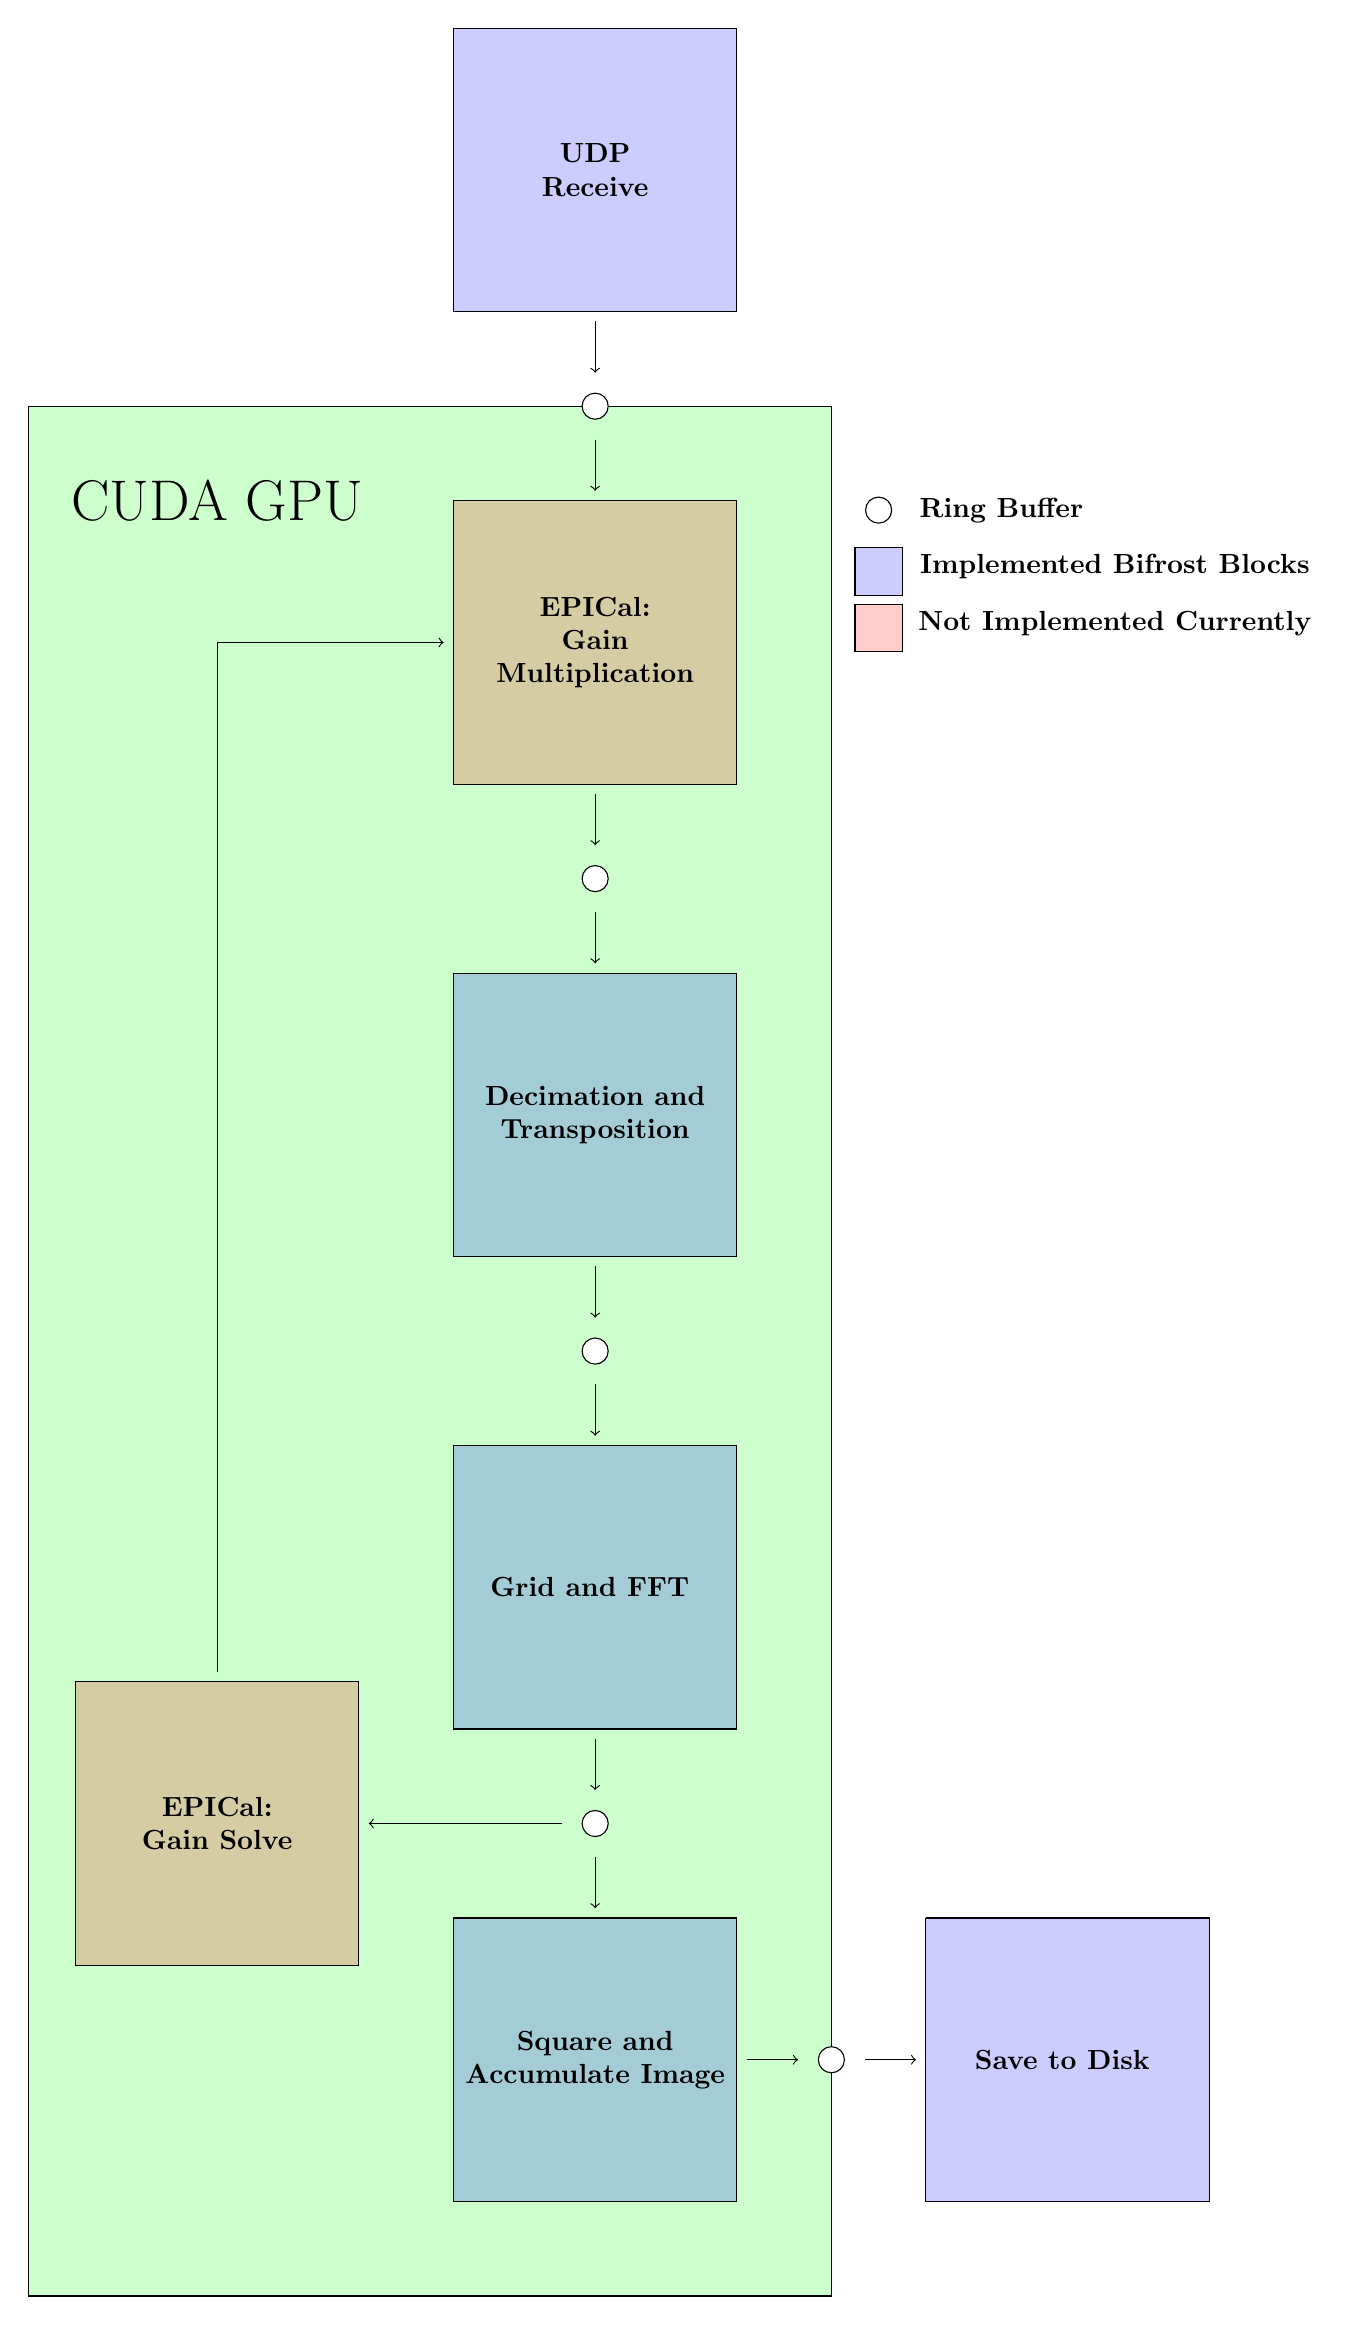
\begin{tikzpicture}[x=1.2cm,y=1.2cm]

  \tikzstyle{every node}=[font=\large, font=\bfseries]
  \draw [fill=blue, fill opacity = 0.2] (0,5.0) -- (3.0,5.0) -- (3.0,5.0 - 3) -- (0,5.0 - 3) -- cycle;
  \node at (1.5,3.5) [align=center] { UDP \\ Receive };
  
  \draw [fill=green, fill opacity = 0.2] (4.0,1.0) -- (4.0,-19) -- (-4.5,-19) -- (-4.5,1.0) -- cycle;

  \draw [fill=red, fill opacity = 0.2] (0,0) -- (3.0,0) -- (3.0,0- 3) -- (0,0 - 3) -- (0,0);
  \foreach \i in {-1,...,-3}
  {
    \draw [fill=blue, fill opacity = 0.2] (0,\i*5) -- (3.0,\i*5) -- (3.0,\i*5 - 3) -- (0,\i*5 - 3) -- (0,\i*5);
  }
  \foreach \i in {1,...,-2}
  {
    \path (1.5,\i*5 - 3) node (y1) {} (1.5,\i*5-3.75) node (y2) {};
    \path (1.5,\i*5 - 4.25) node (y3) {} (1.5,\i*5-5) node (y4) {};
    \draw (1.5,\i*5 - 4) node[circle,style={minimum width=.5ex,fill=white},draw]{};
    \draw [->] (y1) -- (y2);
    \draw [->] (y3) -- (y4);
  }

  \node at (1.5,-1.5) [align=center] { EPICal: \\ Gain  \\ Multiplication };
  \node at (1.5,-6.5) [align=center] { Decimation and \\ Transposition};
  \node at (1.5,-11.5)  [align=center] { Grid and FFT };
  \node at (1.5,-16.5)  [align=center] { Square and \\ Accumulate Image };

  \draw [fill=blue, fill opacity = 0.2] (5.0,-15) -- (8.0,-15) -- (8.0,-18) -- (5.0,-18) -- (5.0,-15);
  \node at (6.5, -16.5) [align = center] { Save to Disk };

  \draw [fill=red, fill opacity = 0.2] (-1.0,-12.5) -- (-4.0,-12.5) -- (-4.0,-15.5) -- (-1.0,-15.5) -- (-1.0,-12.5);
  \node at (-2.5, -14.0) [align = center] { EPICal: \\ Gain Solve };
  \path (1.25,-14.0) node (e1) {} (-1.0,-14.0) node (e2) {};
  \draw [->] (e1) -- (e2);

  \path (3.0,-16.5) node (s1) {} (3.75, -16.5) node (s2) {};
  \path (4.25,-16.5) node (s3) {} (5.0, -16.5) node (s4) {};
  \draw (4.0, -16.5) node[circle,style={minimum width=.5ex,fill=white},draw]{};
  \draw [->] (s1) -- (s2);
  \draw [->] (s3) -- (s4);

  \path (-2.5, -12.5) node (epical1) {} (0,-1.5) node (epical2) {};
  \draw [->] (epical1) |- (epical2);

  \node at (-2.5,0) [align= center, font=\fontsize{20}{1}\selectfont, thick] {CUDA GPU};


  %%% Add key

  \draw (4.5, -0.1) node[circle,style={minimum width=.5ex,fill=white},draw]{};
  \draw (5.8, -0.1) node {Ring Buffer};
  \draw [fill = blue, fill opacity = 0.2] (4.25, -0.5) -- (4.75,-0.5) -- (4.75,-1.0) -- (4.25,-1.0) -- cycle;
  \draw [fill = red, fill opacity = 0.2] (4.25, -1.1) -- (4.75,-1.1) -- (4.75,-1.6) -- (4.25,-1.6) -- cycle;
  \draw (7.0, -0.7) node { Implemented Bifrost Blocks};
  \draw (7.0, -1.3) node { Not Implemented Currently };

  
\end{tikzpicture}
\end{document}
